%%%%%%%%%%%%%%%% Springer %%%%%%%%%%%%%%%%%%%%%%%%%%%%%%%%%%


\documentclass{svproc}
%
% RECOMMENDED %%%%%%%%%%%%%%%%%%%%%%%%%%%%%%%%%%%%%%%%%%%%%%%%%%%
%
\newtheorem{df}{Definition}
\usepackage{amsmath}
\usepackage{array}

\usepackage{color}
\usepackage{graphicx}

\usepackage[numbers,square,sort&compress]{natbib}
\bibliographystyle{spmpsci_unsrt}

% to typeset URLs, URIs, and DOIs
\usepackage{url}
\def\UrlFont{\rmfamily}

\begin{document}
\mainmatter              % start of a contribution
%
\title{Local termination criterion for impulsive component detection using progressive genetic algorithm}
%
\titlerunning{Quantile-based LTC for PGA}  % abbreviated title (for running head)
%                                     also used for the TOC unless
%                                     \toctitle is used
%
 \author{%
 Jacek Wodecki\inst{2},  Anna Michalak\inst{1}, Agnieszka Wy{\l}oma{\'n}ska\inst{1},  Rados{\l}aw Zimroz\inst{2}
}%
%
 \authorrunning{Jacek Wodecki et al.} % abbreviated author list (for running head)
%
%%%% list of authors for the TOC (use if author list has to be modified)
% \tocauthor{Ivar Ekeland, Roger Temam, Jeffrey Dean, David Grove,
% Craig Chambers, Kim B. Bruce, and Elisa Bertino}
%


\institute{ Research and Development Centre, KGHM Cuprum Ltd, Sikorskiego 2-8, 53-659 Wroclaw, Poland \\ \email{\{amichalak, awylomanska\}@cuprum.wroc.pl} \and  Faculty of Geoengineering, Mining and Geology, Diagnostics and Vibro-Acoustic Science Laboratory, Wroclaw University of Science and Technology, Na Grobli 15, 50-421 Wroclaw\\ \email{\{jacek.wodecki, radoslaw.zimroz\}@pwr.wroc.pl}
}

\maketitle              % typeset the title of the contribution

\begin{abstract}
A problem of local damage detection for condition monitoring based on vibration data can be approached from many different angles. One of the most common ways is selective filtration of the vibration signal. There are many techniques allowing to construct digital filter for particular input data (e.g. spectral selectors). In previous articles authors proposed a technique called Progressive Genetic Algorithm (PGA) to optimally design digital filter for a given data set using no prior assumptions. It uses kurtosis as fitness function and local linear fit of fitness function progression vector as a global termination criterion (GTC), but local termination criterion (LTC) was defined as simple stall limit of fitness value. In this paper authors propose a new quantile-based way to terminate PGA locally for faster convergence. Initial testing phase shows that for comparable quality of obtained result, individual epochs terminate significantly faster without sacrificing the progress of local convergence. It results in more efficient optimization and faster global convergence which reduces the overall execution time of the program for about the order of magnitude.
\keywords{genetic algorithm, local damage detection, vibration signal, statistical analysis}
\end{abstract}
%
\section{Introduction}

Analytical methods based on vibration data are very common in machine diagnostics, especially when rotating components are involved. For this class of signals, presence of periodic components is expected, so it is natural to utilize algorithms operating in frequency domain. Machines with rotating components are especially prone to different types of local damage, which is very often manifested as periodic or non-periodic impulsive component placed in unknown frequency band \cite{bartelmus2009new}. Hence, methods aiming in informative frequency band (IFB) detection become very useful \cite{obuchowski2014selection}.

IFB detection methods can incorporate various tools, e.g. statistically justified spectral selectors \cite{obuchowski2014recent,wylomanska2016impulsive,zak20161932}, adaptive filtration \cite{makowski2014new,makowski2013procedure}, time-frequency domain techniques \cite{wodecki2017novel,wylomanska2016application} and many others. Since IFB detection always leads to defining a band (or multiple bands), it can be considered as developing a filter for specific data. If so, one can use prior knowledge about the machine or industrial process to impose various constraints on the algorithm to prepare it as well as possible for the analysis of particular data. Unfortunately, it is rarely the case, so the more general the algorithm, the better for the robustness and reliability.

In previous work authors developed method based on genetic algorithm (GA) for automatic optimal filter design which imposes neither guidance nor constraints that could improve the efficiency of the filter development (see section \ref{pga}) \cite{wodecki2018optimal}. Main difference between this solution and GA-based methods for filter development proposed by other authors is that it describes the concept of progressive genetic algorithm (PGA) that can operate freely without prior information about any expectations. On the other hand, other authors impose constraints or provide other prior information that can guide the filter evolution in predefined direction \cite{nilsson2003digital} or are just trying to refine or simplify the structure of previously known or initially generated filter \cite{lee1998digital,sabbir2006design}. 

Unfortunately, previously implemented local termination criterion (LTC) was based on simple stall with tolerance limit, which resulted in significant waste of time in order to let the current epoch terminate. This article addresses that issue by proposing new and more efficient LTC that is based on evaluation of quantiles of population score after each generation \cite{langford2006quartiles}. Such approach allows the algorithm to react immediately when the population state suggests readiness to terminate the current epoch. 

The rest of the paper is organized as follows: in section \ref{pga} recent work on the development of PGA is reminded, section \ref{crit} explains newly developed LTC based on quantile analysis, section \ref{res} presents obtained results, and finally conclusions are drawn. 


\section{Methodology}

In this section overall methodology of the method is described. Section \ref{pga} reminds the structure of analytical method developed in previous work, and section \ref{crit} describes newly established LTC. 

\subsection{Progressive Genetic Algorithm}\label{pga}

Previously developed method extracts damage-related impulsive component from vibration signal using the idea called Progressive Genetic Algorithm for optimal filter design \cite{wodecki2018optimal}. The main idea is based on the assumption that it is possible to design digital filter using heuristic optimization with kurtosis used as fitness function. Algorithm evolves the population of filter coefficients vectors. The concept of progressiveness assumes extension of vector length, beginning with very short filter that can capture general shape of filter. After a predefined maximum amount of generations, the epoch ends and coefficient vector is extended by 2 entries. This step increases filter precision for the next epoch. Such progressive approach prevents from overfitting and allows the algorithm to pursue more appropriate direction of evolution. 

\subsection{Quantile-based LTC}\label{crit}

In the previous work LTC was defined as simple generation stall limit within certain tolerance for fitness function value. In this form a lot of time was wasted in case when within a single epoch further improvement was non-existent or negligible, while LTC was still supposed to wait for predefined amount of generations to evaluate the stall. 

Main goal of this article is to establish better LTC that omits the stall and terminates the epoch in more appropriate point in time. The core idea is based on the assumption that it is better to analyze the behavior of the entire population than observe only the best individual.

\begin{figure}[ht!]
\centering
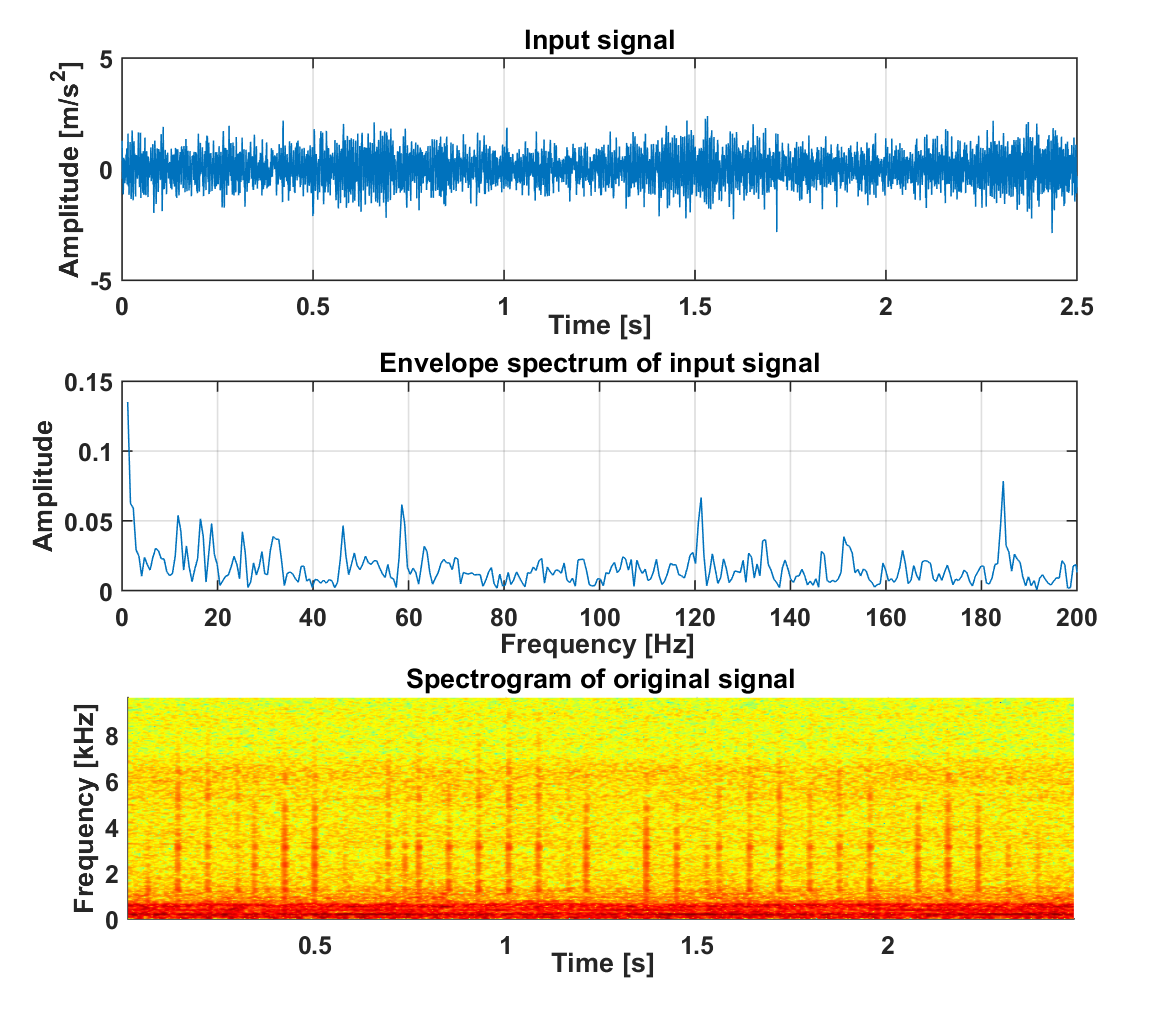
\includegraphics[width=\textwidth]{figs/raw.eps}
\caption{Input vibration data presented in relevant domains}
\label{fig:raw}
\end{figure}

Assume that PGA operates on the population of fixed size $n$. Let $X^{(k)}=\{x^{(k)}_1,x^{(k)}_2,\dots ,x^{(k)}_n\}$ be the vector of fitness function values for the population individuals, evaluated after the $k^{th}$ generation of the given epoch, where $x^{(k)}_1\geq x^{(k)}_2\geq \dots \geq x^{(k)}_n$. For every $k\geq 1$ it is possible to calculate the estimated fitness value $\hat{x}^{(k)}_m$ at $m^{th}$ percentile of the vector $X^{(k)}$, so that:

\begin{equation}
    P\left( X^{(k)}\leq\hat{x}^{(k)}_m \right)\geq \frac{m}{100},
\end{equation}

where by percentile authors unterstand the quantile of the order 100. LTC will terminate the given epoch after $k^{th}$ generation if $\hat{x}^{(k)}_m$ reaches the value of $x^{(k)}_1$. In practice $1\%$ uncertainty is implemented so termination occurs if  $\hat{x}^{(k)}_m\geq 0.99*x^{(k)}_1$.


\section{Results}\label{res}

In this section authors verify the results of presented method using real single-channel vibration data from damaged rolling bearing (see Fig \ref{fig:raw}). It is the same signals as in the preceding article with initial kurtosis value equal to 3.09 \cite{wodecki2018optimal}. Sampling frequency equals 19.2 kHz. It is known that wideband impulsive component with modulation frequency of 12.7 Hz is expected to be discovered, which corresponds to local damage of the outer race of the bearing.

Testing methodology assumes running the algorithm on the same machine using identical real-life data with fixed random seed to eliminate the random aspects of the algorithm i.e. generation of population individuals, occurrence of random mutations, behavior of heuristic crossover etc.


Parameters of designed real-coded PGA are presented in Table \ref{tab:tab1}.

\begin{table}[ht!]
    \centering
    \caption{Parameters of PGA}
    \begin{tabular}{|l|l|}
    \hline
         \textbf{Parameter} & \textbf{Value} \\ \hline
         Initial filter length & 7 \\ \hline
         Population size & 150 \\ \hline
         Termination criterion & NRMSE \\ \hline
         Generations per epoch & 80 \\ \hline
         Initial population & Random $\sim$ N(0,1) \\ \hline
         Selection & Roulette \\ \hline
         Crossover & Heuristic with d=1.5 \\ \hline
         Mutation & Uniform with R=0.01 \\ \hline
         Elite individuals & 3 \\ \hline
         Stall limit & 20 \\ \hline
         Average change for stall limit & $10^{-6}$ \\ \hline
         LTC quantile & 5\% \\
    \hline
    \end{tabular}
    \label{tab:tab1}
\end{table}

It is important to note that stall limit and average change for stall limit are taken into consideration only when the previously used stall-based LTC (SLTC) is tested, and LTC quantile only concerns the case when quantile-based LTC (QLTC) is tested.

Input data has been fed into the PGA twice, once for each LTC, and let alone until GTC terminates the algorithm. Fig. \ref{fig:progress} presents the behavior of the algorithm using both LTC's. There are several arguments that it provides in favor of the QLTC:

\begin{figure}[ht!]
\centering
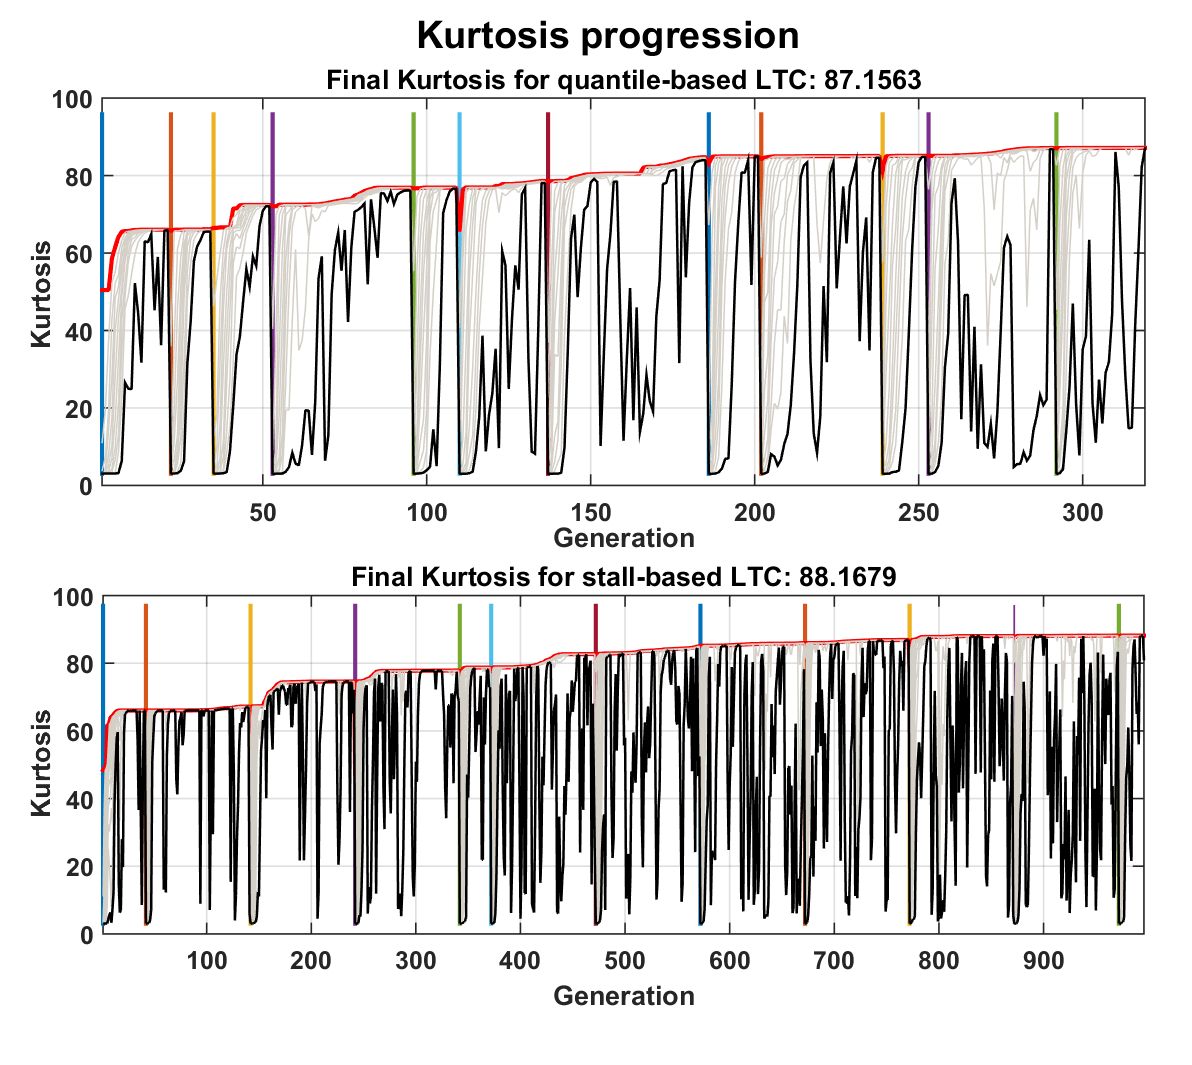
\includegraphics[width=\textwidth]{figs/progress.eps}
\caption{Fitness function progression (red) with 5\% percentile (black), other percentiles at multiples of 10\% (gray) and borders between consecutive epochs (vertical lines)}
\label{fig:progress}
\end{figure}

\begin{itemize}
    \item Final values of kurtosis achieved by obtained filters are very similar and the difference between them is negligible on this scale;
    \item The amount of processed epochs is identical, so evolved filters have the same amount of coefficients, which translates into equal capabilities in terms of filter precision;
    \item In opposition to SLTC, for QLTC one cannot observe significantly long segments of time where quantile reached the value of fitness function and remained there for some time. Such segments are not useful for the evolution and in general in such case the time is wasted. One could argue that in such periods a random mutation could occur and make a difference, but since it is theoretically unpredictable when then mutation takes place, such idea carries no meaning in this context;
    \item Since both results share all the qualitative features, it is clear that significantly lower amount of total generations in case of QLTC test becomes the great advantage in terms of computational time and overall efficiency of the algorithm as a whole. 
\end{itemize}

\begin{figure}[ht!]
\centering
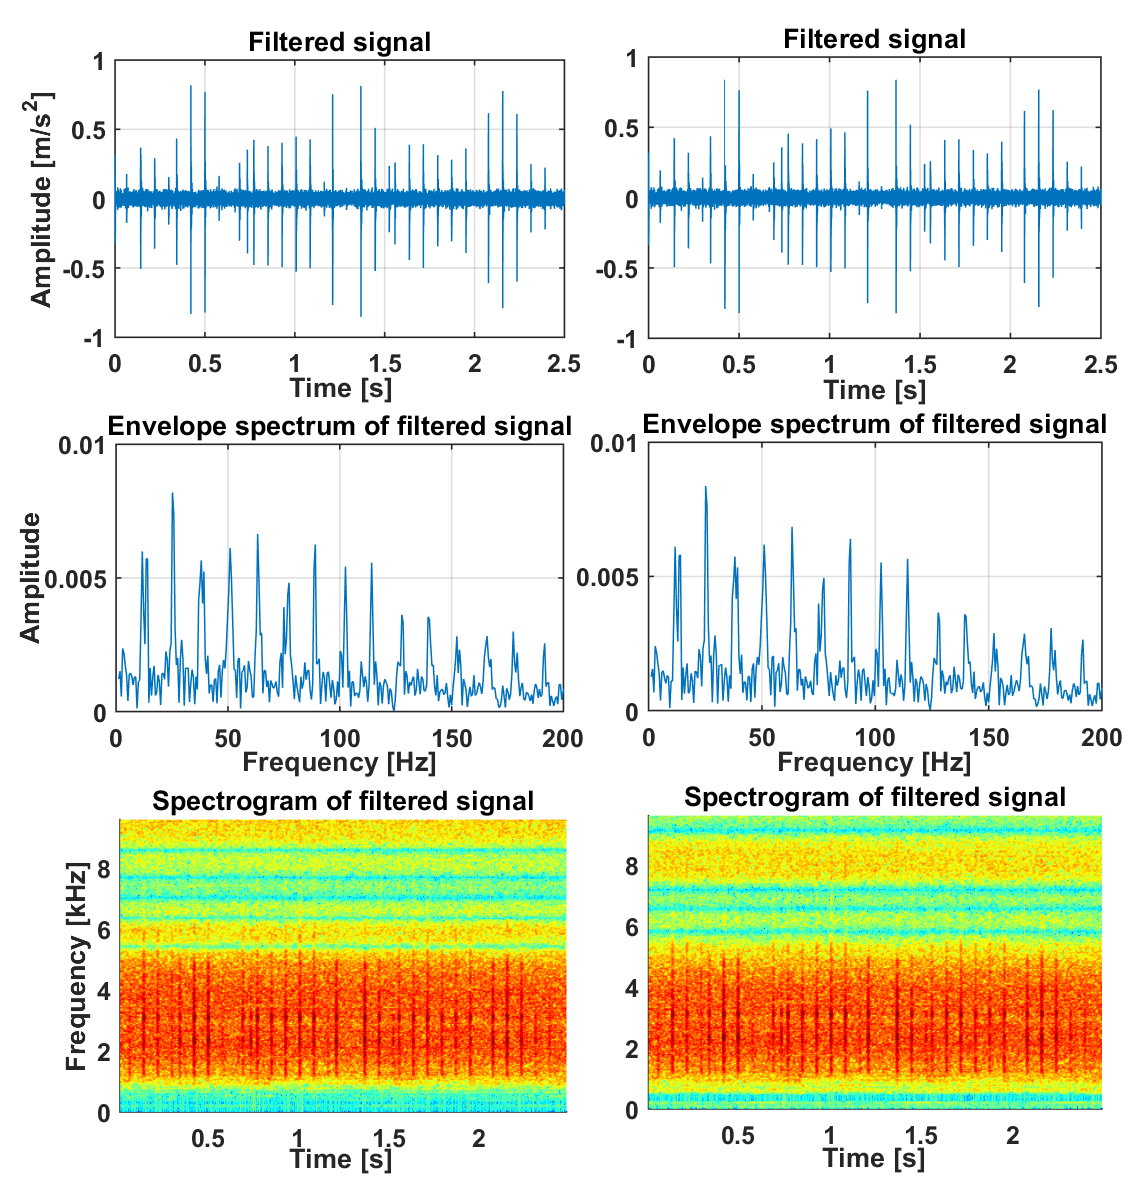
\includegraphics[width=\textwidth]{figs/result.eps}
\caption{Results of filtration using obtained filters. Left - QLTC, right - SLTC}
\label{fig:result}
\end{figure}

Finally, SLTC test needed 997 iterations to complete, which translates into 906 seconds or 15.1 minutes. On the other hand, QLTC test achieved the result in 319 iterations, which makes 266 seconds or 4.43 minutes. Hence, time as well as amount of generations needed was reduced by 71\%.



Figure \ref{fig:result} presents output signals obtained after processing with evolved filters. It is clear that qualitatively signals are filtered equivalently well. Plots of time series and envelope spectrum are practically indistinguishable. Spectrograms on the other hand reveal slight differences between two results. In general both filters were able to correctly identify main IFB mode roughly between 1 kHz and 5 kHz. Though, filter produced by QLTC provides more pronounced cutoff between main IFB mode and lower frequencies, which in the raw signal carry a lot of highly energetic components that do not contain information about the impulses. Frequency bands above 5 kHz are differently shaped for both results, but it affects neither the noise floor level nor the informativeness carried by time series or envelope spectrum.

\section{Conclusions}

In this paper authors introduce new approach for local termination criterion of progressive genetic algorithm used in the application of local damage detection in rotating machinery. As a general principle, recently developed concept of progressive genetic algorithm is used for unconstrained optimal filter design. In opposition to previously used SLTC, new QLTC allows for more intelligent epoch termination that results in faster evolution without sacrificing the quality of obtained results. Performance was tested in fixed numerical conditions using real-life vibration signal from damaged ball bearing.

\bibliography{mybibfile}


\end{document}
